\chapter{Estado del Arte}\label{background}

\section{Consideraciones Iniciales}

La detección precisa del tiempo de llegada de las fases sísmicas, especialmente la onda P (P-wave), constituye un componente crítico en múltiples aplicaciones dentro de la sismología, como la localización de eventos sísmicos, la estimación de magnitud, y la caracterización de la estructura del subsuelo. La calidad de esta detección influye directamente en la eficiencia de los sistemas de alerta temprana (EEWS, por sus siglas en inglés), así como en la calidad de los catálogos sísmicos utilizados para el análisis tectónico y de peligrosidad.

Históricamente, se han empleado métodos clásicos para la identificación de la llegada de la onda P, entre los que destacan el algoritmo STA/LTA (Short-Term Average over Long-Term Average) y el método AIC (Criterio de Información de Akaike). El método STA/LTA se basa en la comparación entre dos ventanas temporales —una de corto plazo y otra de largo plazo— aplicadas a la señal sísmica; si la razón entre ambas supera un umbral definido, se considera como una posible llegada de la fase P \cite{zhang2020first} \cite{kalkan2016automatic}. Por otro lado, el método AIC segmenta la señal considerando que los intervalos antes y después del arribo de la onda pertenecen a procesos estadísticos distintos, seleccionando como punto de quiebre el que minimiza la función AIC \cite{shang2018enhancing}.

Si bien estos enfoques tradicionales han demostrado utilidad en múltiples contextos, presentan limitaciones importantes en entornos con baja relación señal-ruido (SNR), presencia de ruido impulsivo, o configuraciones con sensores de baja calidad. Estas limitaciones han motivado el desarrollo de enfoques más avanzados y robustos.

En la última década, el campo ha sido testigo de un crecimiento sostenido en el uso de técnicas de aprendizaje automático y aprendizaje profundo para la detección de fases sísmicas. Modelos como redes neuronales artificiales (RNA), redes convolucionales (CNN), arquitecturas híbridas (CNN+LSTM) y, más recientemente, arquitecturas basadas en Transformers, han sido aplicadas para extraer automáticamente características relevantes de los registros sísmicos. Estos modelos buscan superar las limitaciones de los métodos clásicos, ofreciendo mayor precisión, adaptabilidad y tolerancia al ruido.

Algunos trabajos destacados en esta línea incluyen el uso de representaciones espectrales como entrada para redes neuronales artificiales, la extracción multiescala mediante EMD (Descomposición Modal Empírica), y arquitecturas profundas como PhaseNet \cite{10.1093/gji/ggy423}, EQTransformer \cite{mousavi2019cred}, TransQuake \cite{zhang2023ept} e ICAT-net \cite{Bertino93}. Estos modelos han logrado resultados prometedores en tareas de picking automático, incluso en contextos de datos limitados o condiciones ambientales adversas.

En esta tesis se adopta una perspectiva comparativa, evaluando la efectividad de estos métodos tanto clásicos como modernos para la detección de la onda P (y en algunos casos la onda S), con énfasis en su aplicabilidad en entornos con recursos computacionales restringidos. Esta visión parte del reconocimiento de que, si bien los modelos complejos ofrecen ventajas en precisión, su uso en dispositivos embebidos o redes distribuidas requiere soluciones ligeras y generalizables.

La detección precisa del tiempo de llegada de la onda P (P-Wave) es crucial para diversos estudios sísmicos, incluyendo la localización de terremotos, la estimación de la magnitud y la evaluación de la estructura del subsuelo. En este contexto, se han desarrollado diversos métodos para identificar el inicio de la onda P en registros sísmicos.

Entre los métodos clásicos se encuentran el selector STA/LTA (Relación Corto Plazo / Largo Plazo) y el selector AIC (Criterio de Información de Akaike). El método STA/LTA calcula una función característica basada en la proporción entre una ventana de corto plazo y una ventana de largo plazo. Si esta fracción supera un umbral establecido, se considera la presencia de una onda P \cite{zhang2020first} \cite{kalkan2016automatic}. Por otro lado, el método AIC asume que los intervalos antes y después de la llegada de la onda P representan dos procesos estacionarios diferentes. Este método minimiza la función AIC para determinar el momento preciso de la llegada de la onda P \cite{shang2018enhancing}.

\section{Tema 1: Metodo STA/LTA}

El algoritmo STA/LTA (Short-Term Average / Long-Term Average) es uno de los métodos clásicos más ampliamente utilizados para la detección automática de eventos sísmicos, en particular para el picking de la primera llegada de la onda P. Su popularidad radica en su bajo costo computacional, facilidad de implementación, y su capacidad para operar en tiempo real, incluso en estaciones sísmicas remotas o portátiles con capacidades limitadas \cite{allen1978automatic}.

El principio del método es relativamente simple: consiste en calcular en tiempo real dos promedios móviles sobre la señal sísmica filtrada —uno de corto plazo (STA) y otro de largo plazo (LTA)— y evaluar la razón entre ambos. El valor de STA se asocia con los cambios inmediatos o transitorios en la amplitud de la señal, mientras que el valor de LTA refleja el nivel promedio del ruido de fondo. Cuando la razón STA/LTA supera un umbral predefinido, se considera que ha ocurrido un cambio significativo en la señal, posiblemente asociado con el arribo de una fase sísmica \cite{allen1978automatic}.

\subsection{Mejoras Basadas en Umbrales de Referencia}

En su trabajo más reciente, \cite{qiu2023sta} proponen una mejora sustancial del método STA/LTA clásico mediante la introducción de un umbral de referencia adaptativo, basado en el nivel de ruido de fondo \cite{qiu2023sta}. La idea principal consiste en establecer una relación cuantitativa entre el umbral de disparo y la estadística del ruido previo al evento, eliminando así la necesidad de ajustes empíricos arbitrarios.

Para ello, los autores utilizan una función característica basada en la relación señal/ruido (SNR), que permite discriminar más eficazmente los arrivos sísmicos verdaderos del ruido aleatorio. Además, proponen dos versiones del algoritmo:

\begin{itemize}
    \item STA/LTA basado en umbral de referencia: Se calcula un umbral dinámico a partir de la estadística de la ventana LTA, tomando en cuenta desviación estándar o percentiles del ruido \cite{qiu2023sta}.
    \item STA/LTA mejorado con ventana cancelable: En escenarios donde se presentan ruidos impulsivos breves que podrían disparar erróneamente el algoritmo, se mejora la posición de la ventana STA y se introduce una lógica que anula temporalmente la ventana si se detecta una anomalía \cite{qiu2023sta}.
\end{itemize}

Estas mejoras logran una mayor robustez frente al ruido ambiental, adaptabilidad ante distintos tipos de registros, y mayor precisión sin necesidad de calibración manual. Los autores validan su propuesta con datos reales, mostrando una mejora significativa en comparación con el STA/LTA tradicional tanto en términos de exactitud como de precisión \cite{qiu2023sta}.

\subsection{Extensión Fractal del STA/LTA}

Por su parte, \cite{zhang2018sta} proponen una extensión innovadora basada en el uso de la dimensión fractal como característica de la señal \cite{zhang2018sta}. Su hipótesis parte del hecho de que las señales sísmicas reales presentan propiedades fractales distintas antes y después de la llegada de una fase sísmica. Al integrar esta métrica dentro de las ventanas de análisis del algoritmo STA/LTA, es posible detectar con mayor sensibilidad los puntos de quiebre.

La dimensión fractal se calcula usando el método de caja cuadrada (box-counting) o variantes similares, y se integra como una función secundaria que refuerza la decisión del disparador \cite{zhang2018sta}. En entornos donde el cambio de energía no es suficientemente abrupto como para afectar la STA/LTA de manera directa (por ejemplo, en sismos lejanos o enterrados), la dimensión fractal permite identificar un cambio estructural en la señal \cite{zhang2018sta}.

Esta combinación ha mostrado buenos resultados en bases de datos con señales ruidosas o de baja amplitud, y representa una solución intermedia entre los métodos clásicos deterministas y los modelos complejos de aprendizaje profundo \cite{zhang2018sta}.

En años recientes, se han desarrollado métodos más sofisticados basados en el aprendizaje automático, como el selector basado en EMD (Descomposición Modal Empírica), la identificación mediante RNA (Red Neuronal Artificial), XTF-CNN, CNN (Red Neuronal Convolucional) y CPIC. Estos métodos utilizan técnicas de aprendizaje automático para extraer características relevantes de los registros sísmicos y así identificar el inicio de la onda P con mayor precisión y robustez \cite{zhu2019deep} \cite{bi2021explainable} \cite{zhang2018sta}.

\section{Tema 2: Metodo Basado en Redes Convolucionales}

Los métodos basados en redes convolucionales (CNN) han ganado popularidad en el procesamiento de señales sísmicas debido a su capacidad para extraer características discriminativas de datos complejos y ruidosos. A continuación, se presentan dos trabajos relevantes que aplican arquitecturas convolucionales al problema de la detección y clasificación de fases sísmicas.

\subsection{Aplicación de redes convolucionales a la detección y selección de fases teleseísmicas: casos PcP y PKiKP}

En el estudio realizado por \cite{khattak2024conveq}, se propone una red convolucional para la detección y clasificación de fases sísmicas teleseísmicas, en particular las fases PcP y PKiKP \cite{zhu2023teleseismic}. La arquitectura de la red de detección está basada en una CNN clásica (LeCun et al., 1998), diseñada para identificar fases sísmicas latentes a partir de segmentos de forma de onda de 20 segundos, muestreados a 100 Hz (2000 muestras por entrada).

La red de detección consta de una pila de cuatro capas convolucionales seguidas de una capa totalmente conectada, la cual estima probabilidades para tres clases: \textit{good}, \textit{fair} y \textit{poor}. Se utiliza una función de pérdida de entropía cruzada y se aplica el algoritmo ADMM (Alternating Direction Method of Multipliers) para la optimización de los pesos de la red, con una tasa de aprendizaje de $0.0001$. Para prevenir el sobreajuste se implementa la técnica de \textit{dropout} después de cada capa de \textit{pooling} y capa densa. El conjunto de entrenamiento incluye 7000 sismogramas, de los cuales se derivan 6000 fases etiquetadas balanceadamente entre las tres clases, logrando tasas de detección de hasta 94\% para fases PKiKP.

Posteriormente, las fases clasificadas como \textit{good} o \textit{fair} son procesadas por una red de \textit{picking}, diseñada para localizar el \textit{first break} o inicio de la fase sísmica. Esta red está inspirada en una red totalmente convolucional (FCN) utilizada originalmente para segmentación de estructuras celulares (Ronneberger et al., 2015). La arquitectura FCN sigue un esquema en forma de \textit{U}, con una ruta contráctil para extraer características de bajo nivel, y una ruta expansiva para proyectarlas en una salida de alta resolución que representa la probabilidad de ocurrencia del inicio de la fase.

Cada \textit{first break} es representado con una distribución Gaussiana de desviación estándar 20 ms, lo que facilita la convergencia del modelo. La función de pérdida utilizada es también de entropía cruzada, optimizada mediante ADMM. Los resultados muestran que las pérdidas de validación convergen a casi cero en menos de 100 épocas, demostrando una alta eficacia en el entrenamiento.

\subsection{ConvEQ: Clasificación de fases sísmicas usando redes convolucionales y transformada de frecuencia de tiempo corto}

Otra contribución relevante es el modelo \textit{ConvEQ}, que implementa una red convolucional para la clasificación automática de fases sísmicas a partir de transformadas en frecuencia de corto tiempo (STFT) \cite{khattak2024conveq}. El diseño de la red se basa en una arquitectura CNN con tres capas convolucionales, seguidas por funciones de activación ReLU, normalización por lotes (\textit{batch normalization}), y capas de \textit{dropout} con tasa de 20\%.

El objetivo principal de la red es extraer características significativas a partir de representaciones en tiempo-frecuencia de las señales sísmicas. Tras las convoluciones, una capa densa captura la información discriminativa para la clasificación de las fases. Finalmente, una capa de salida con funciones de activación softmax proporciona una probabilidad para cada clase, seleccionando aquella con mayor probabilidad como resultado.

La arquitectura fue optimizada a través de estudios de ablación detallados, ajustando hiperparámetros como número de filtros, tamaño del kernel y profundidad de la red. Los resultados demuestran que la red ConvEQ es robusta y computacionalmente eficiente, siendo capaz de clasificar eventos sísmicos incluso en condiciones de bajo SNR.

\section{Tema 3: Métodos Basados en Redes Transformer}

En los últimos años, las arquitecturas basadas en Transformers han emergido como una herramienta poderosa en el procesamiento de señales sísmicas, debido a su capacidad para modelar relaciones de largo alcance en los datos y su flexibilidad para adaptarse a diferentes tareas. Uno de los modelos más destacados en este ámbito es EQTransformer \cite{mousavi2019cred}, que combina redes convolucionales (CNN), redes recurrentes bidireccionales (BiLSTM) y mecanismos de atención para la detección y clasificación de fases sísmicas.

\subsection{EQTransformer: Arquitectura y Aplicaciones}

EQTransformer es un modelo híbrido diseñado para realizar detección, clasificación y picking de fases sísmicas en un solo pipeline. La arquitectura del modelo consta de tres componentes principales:

\begin{itemize}
    \item \textbf{Extracción de características locales:} Se utilizan capas convolucionales para capturar patrones locales en las formas de onda sísmicas.
    \item \textbf{Modelado de dependencias temporales:} Las capas BiLSTM permiten modelar relaciones temporales de largo alcance en los datos.
    \item \textbf{Mecanismo de atención:} Este componente asigna pesos a diferentes partes de la señal, destacando las regiones más relevantes para la tarea de detección.
\end{itemize}

El modelo es entrenado utilizando grandes conjuntos de datos sísmicos etiquetados, como el dataset STEAD, y ha demostrado un rendimiento sobresaliente en la detección de fases P y S, incluso en condiciones de bajo ruido-señal (SNR). Además, EQTransformer es capaz de generalizar a diferentes regiones geográficas y configuraciones de sensores, lo que lo convierte en una herramienta versátil para aplicaciones sísmicas.

\subsection{Limitaciones y Desafíos}

A pesar de sus ventajas, EQTransformer presenta algunas limitaciones. Su alto costo computacional y la necesidad de hardware especializado dificultan su implementación en dispositivos embebidos o estaciones sísmicas con recursos limitados. Además, el modelo requiere grandes volúmenes de datos etiquetados para su entrenamiento, lo que puede ser un desafío en regiones con datos limitados o no etiquetados.

\subsection{Comparación con Otros Modelos Basados en Transformers}

En comparación con otros modelos basados en Transformers, como TransQuake \cite{zhang2023ept} e ICAT-net \cite{Bertino93}, EQTransformer destaca por su enfoque integral y su capacidad para realizar múltiples tareas en un solo pipeline. Sin embargo, modelos más recientes como ICAT-net han sido diseñados específicamente para entornos con recursos computacionales restringidos, lo que los hace más adecuados para aplicaciones en tiempo real o en dispositivos embebidos.

En esta tesis, se evalúa el desempeño de EQTransformer y otros modelos basados en Transformers en la detección de fases sísmicas, con énfasis en su aplicabilidad en entornos con recursos limitados. Los resultados obtenidos permitirán identificar las fortalezas y debilidades de estos enfoques, así como proponer mejoras para su implementación en sistemas de alerta temprana y análisis sísmico.

\section{Tema 4: Modelos Híbridos y Avances Recientes}
En los últimos años, se han desarrollado modelos híbridos que combinan diferentes arquitecturas y enfoques para mejorar la detección de fases sísmicas. Estos modelos buscan aprovechar las fortalezas de cada técnica para superar las limitaciones individuales y ofrecer soluciones más robustas y precisas.

\subsection{PhaseNet: Red Neuronal Convolucional para Detección de Fases Sísmicas}
PhaseNet es un modelo basado en redes neuronales convolucionales (CNN) diseñado específicamente para la detección automática de fases sísmicas, como las ondas P y S. Este modelo utiliza una arquitectura de red profunda que combina múltiples capas convolucionales para extraer características relevantes de las formas de onda sísmicas. PhaseNet ha demostrado ser efectivo en la identificación de fases sísmicas en registros ruidosos y ha sido validado en diferentes regiones geográficas, mostrando una alta precisión y robustez en la detección de eventos sísmicos \cite{10.1093/gji/ggy423}.

\begin{figure}[htbp]
    \centering
    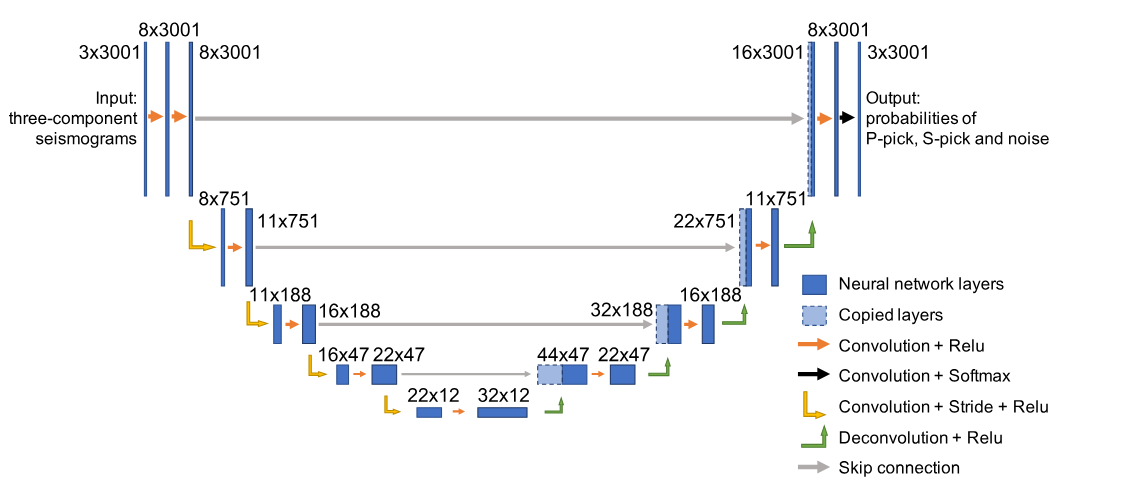
\includegraphics[width=0.8\textwidth]{figures/POHASENET.png}
    \caption{Arquitectura de PhaseNet \cite{10.1093/gji/ggy423}.}
    \label{fig:phasenet_architecture}
\end{figure}

\subsection{TransQuake: Modelo Híbrido para Detección de Eventos Sísmicos}
TransQuake es un modelo híbrido que combina redes convolucionales (CNN) y Transformers para la detección precisa y generalizable de eventos sísmicos. Este modelo se basa en la idea de que las redes convolucionales son efectivas para capturar patrones locales en las formas de onda, mientras que los Transformers son capaces de modelar relaciones de largo alcance en los datos. TransQuake ha demostrado ser más eficiente que modelos anteriores como EQTransformer, logrando una mayor precisión en la detección de eventos sísmicos con un menor costo computacional \cite{zhang2023ept}.

\begin{table*}[htbp]
\centering
\caption{Principales Modelos existentes}
\begin{tabular}{p{3cm}p{4.2cm}p{4.2cm}p{3cm}}
\hline
\textbf{Trabajo} & \textbf{Contribución Principal} & \textbf{Limitaciones} & \textbf{Relevancia para esta tesis} \\
\hline
\textbf{STA/LTA} & Método tradicional basado en relaciones de promedios para detección de eventos sísmicos & Alta tasa de falsos positivos en entornos ruidosos y baja SNR & Baja: sirve como referencia de métodos clásicos \\
\hline
\textbf{PhaseNet} & Red neuronal convolucional para identificación automática de fases P y S & Necesita datos etiquetados con precisión y reentrenamiento para nuevas regiones & Alta: pionero en uso de deep learning en sismología \\
\hline
\textbf{EQTransformer} & Modelo híbrido CNN + BiLSTM + atención para detección y picking en un solo pipeline & Alto costo computacional, requiere hardware potente & Alta: enfoque integral para EEWS, pero limitado en dispositivos con pocos recursos \\
\hline
\textbf{TransQuake} & Uso de Transformers para detección precisa y generalizable de eventos sísmicos & Sensible a hiperparámetros y requiere suficientes datos de entrenamiento & Alta: modelo robusto y más eficiente que EQTransformer \\
\hline
\textbf{ICAT-net} & Arquitectura ligera con atención espacial y de coordenadas más componente transformer & Falta validación en diversos contextos reales; limitada caracterización de fuentes sísmicas & Muy Alta: orientado a dispositivos embebidos y entornos con recursos limitados \\
\hline
\textbf{ConvEQ} & Red convolucional para clasificación de fases sísmicas usando STFT & Limitado a datos con alta calidad y resolución; no aborda picking & Media: útil para clasificación, pero no para picking \\
\end{tabular}
\label{tab:trabajos_relacionados}
\end{table*}


\begin{table*}[htbp]
 \centering
  \caption{Tabla de comparacion entre modelos para deteccion de fase P usando los datos de la Station CI.DJJ, CI.DEC, CI.RIN, CI.LFP, 1000 datos para evaluacion (el dataset de entrenamiento fue el mismo especificado por el paper de procedencia)} \label{tabla-1}
 {\small
 \begin{tabular}{ccccccc}
  \hline
  \hline
  \thead{Modelo} & \thead{Pr} & \thead{Re} & \thead{F1} & \thead{Training data} &  \thead{Training Size} & \thead{Ref.}\\
  \hline
  \hline
  P picker by \\ Transformers & $0.89$ & $0.89$ & $0.89$ & $STEAD$ & $700k$ & \cite{Mousavi2020} \\
  \hline
  PhaseNet & $0.89$ & $0.89$ & $0.89$ & $Canada$ & $700k$ & \cite{10.1093/gji/ggy423} \\
  \hline
  GPD & $0.81$ & $0.80$ & $0.81$ & $Canada$ & $4.5M$ & \cite{Ross_2018} \\
  \hline
  PickNet & $0.81$ & $0.49$ & $0.61$ & $Japan Station$ & $740K$ & \cite{WangAndXiao} \\
  \hline
  PpkNet & $0.90$ & $0.90$ & $0.90$ & $Japan Station$ & $30K$ & \cite{ZhouAndYijian} \\
  \hline
  Yews & $0.54$ & $0.72$ & $0.61$ & $Taiwan Station$ & $1.4M$ & \cite{ZHU2019106261} \\
  \hline
  Kurtosis & $0.94$ & $0.79$ & $0.86$ & $--$ & $--$ & \cite{saragiotis2002pai} \\
  \hline
  FilterPicker & $0.95$ & $0.82$ & $0.88$ & $--$ & $--$ & \cite{lomax2012automatic} \\
  \hline
  AIC & $0.92$ & $0.83$ & $0.87$ & $--$ & $--$ & \cite{maeda1985method} \\
  \hline
  
  \hline
 \end{tabular}}
\end{table*}


\begin{table*}[htbp]
 \centering
  \caption{Tabla de comparacion entre modelos para deteccion de fase S usando los datos de la Station CI.DJJ, CI.DEC, CI.RIN, CI.LFP, 1000 datos para evaluacion (el dataset del entrenamiento fue el mismo especificado por el paper de procedencia)} \label{tabla-2}
 {\small
 \begin{tabular}{ccccccc}
  \hline
  \hline
  \thead{Modelo} & \thead{Pr} & \thead{Re} & \thead{F1} & \thead{Training data} &  \thead{Training Size} & \thead{Ref.}\\
  \hline
  \hline
  P picker by \\ Transformers & $0.86$ & $0.86$ & $0.86$ & $Canada$ & $700k$ & \cite{Mousavi2020} \\
  \hline
  PhaseNet & $0.85$ & $0.85$ & $0.85$ & $Canada$ & $700k$ & \cite{10.1093/gji/ggy423} \\
  \hline
  GPD & $0.81$ & $0.83$ & $0.82$ & $Canada$ & $4.5M$ & \cite{Ross_2018} \\
  \hline
  PickNet & $0.75$ & $0.75$ & $0.75$ & $Japan Station$ & $740K$ & \cite{WangAndXiao} \\
  \hline
  PpkNet & $0.95$ & $0.90$ & $0.93$ & $Japan Station$ & $30K$ & \cite{ZhouAndYijian} \\
  \hline
  Yews & $0.83$ & $0.55$ & $0.66$ & $Taiwan Station$ & $1.4M$ & \cite{ZHU2019106261} \\
  \hline
  Kurtosis & $0.89$ & $0.39$ & $0.55$ & $--$ & $--$ & \cite{saragiotis2002pai} \\
  \hline
  FilterPicker & $0.61$ & $0.41$ & $0.49$ & $--$ & $--$ & \cite{lomax2012automatic} \\
  \hline
  AIC & $0.87$ & $0.51$ & $0.64$ & $--$ & $--$ & \cite{maeda1985method} \\
  \hline
  
  \hline
 \end{tabular}}
\end{table*}

\begin{table*}[htbp]
 \centering
  \caption{Tabla de comparacion entre modelos para deteccion de inicio de fase usando los datos de la Station CI.DJJ, CI.DEC, CI.RIN, CI.LFP, 1000 datos para evaluacion (el entrenamiento fue el mismo especificado por el paper de procedencia) En este caso los modelos DetNet y Yews fueron modelos preentrenados con diferentes datasets, STA/LTA es el algoritmo recursivo. Los modelos P picker by Transformer y CRED, son modelos transformers entrenados con el STEAD} \label{tabla-3}
 {\small
 \begin{tabular}{ccccccc}
  \hline
  \hline
  \thead{Modelo} & \thead{Pr} & \thead{Re} & \thead{F1} & \thead{Training data} &  \thead{Training Size} & \thead{Ref.}\\
  \hline
  \hline
  P picker by \\ Transformers & $1.0$ & $0.96$ & $0.98$ & $GLOBAL$ & $1.2M$ & \cite{Mousavi2020} \\
  \hline
  CRED & $1.0$ & $0.96$ & $0.98$ & $GLOBAL$ & $1.2M$ & \cite{mousavi2019cred} \\
  \hline
  DetNet & $1.0$ & $0.89$ & $0.94$ & $China$ & $30K$ & \cite{ZhouAndYijian} \\
  \hline
  Yews & $0.84$ & $0.85$ & $0.85$ & $Taiwan$ & $1.4M$ & \cite{ZHU2019106261} \\
  \hline
  STA/LTA & $0.91$ & $1.0$ & $0.95$ & $--$ & $--$ & \cite{allen1978automatic} \\
  \hline
  
  \hline
 \end{tabular}}
\end{table*}
